\documentclass{article}
\usepackage{graphicx}
\usepackage{geometry}
\usepackage{hyperref}
\usepackage{booktabs}
\usepackage{subcaption}
\usepackage{amsmath}

\geometry{
    a4paper,
    margin=0.65in
}

\hypersetup{
    colorlinks=true,
    linkcolor=blue,
    filecolor=magenta,      
    urlcolor=cyan,
}

\title{Convolutional Neural Network (CNN) Baseline\\Learning Rate Sweeps under Data Heterogeneity and Attacks}
\author{ByzFL SNN Benchmark}
\date{\today}

\begin{document}

\maketitle

\clearpage
\tableofcontents
\clearpage

\section{Introduction}
This report documents the robustness sweeps of standard Convolutional Neural Networks (CNN) using various Learning Rates.

\clearpage

\section{Best Overall Performance (Worst-Case Across Attacks)}
\begin{figure}[htbp]
    \centering
    \begin{subfigure}[b]{0.24\textwidth}
        \centering
        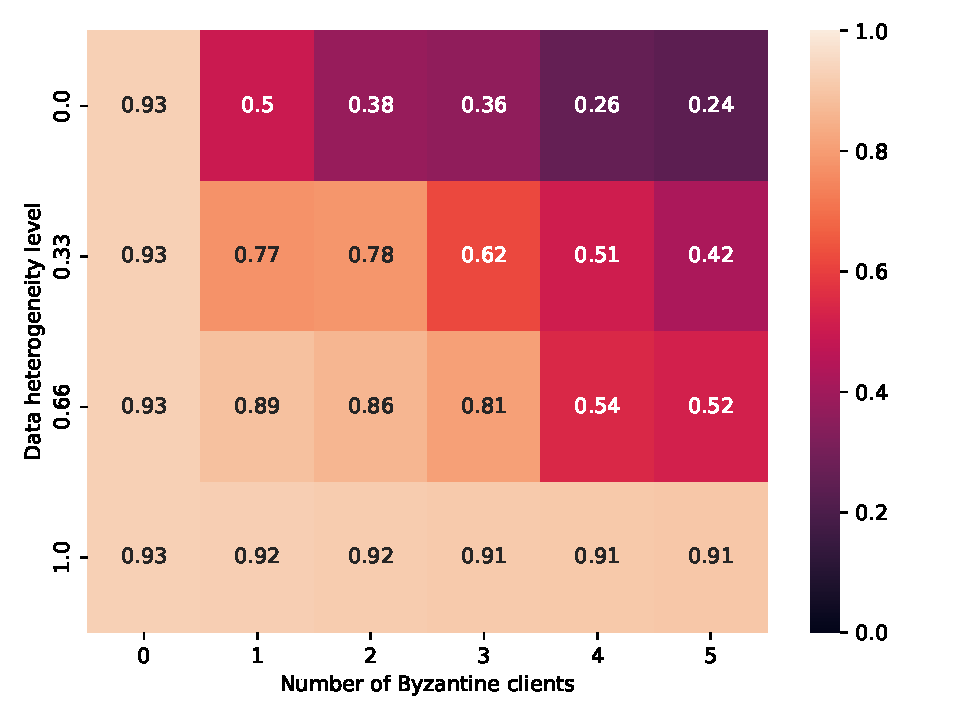
\includegraphics[width=\textwidth]{../plots/robust_comparison_sweep/learning_rate_0.01/best_test_mnist_cnn_mnist_gamma_similarity_niid_NNM_ARC_nb_honest_clients_10_tolerated_f_equal_real.pdf}
        \caption{$\text{LR} = 0.01$}
        \label{fig:best_overall_lr_0_01}
    \end{subfigure}
    \hfill
    \begin{subfigure}[b]{0.24\textwidth}
        \centering
        \includegraphics[width=\textwidth]{../plots/robust_comparison_sweep/learning_rate_0.05/best_test_mnist_cnn_mnist_gamma_similarity_niid_NNM_ARC_nb_honest_clients_10_tolerated_f_equal_real.pdf}
        \caption{$\text{LR} = 0.05$}
        \label{fig:best_overall_lr_0_05}
    \end{subfigure}
    \hfill
    \begin{subfigure}[b]{0.24\textwidth}
        \centering
        \includegraphics[width=\textwidth]{../plots/robust_comparison_sweep/learning_rate_0.08/best_test_mnist_cnn_mnist_gamma_similarity_niid_NNM_ARC_nb_honest_clients_10_tolerated_f_equal_real.pdf}
        \caption{$\text{LR} = 0.08$}
        \label{fig:best_overall_lr_0_08}
    \end{subfigure}
    \hfill
    \begin{subfigure}[b]{0.24\textwidth}
        \centering
        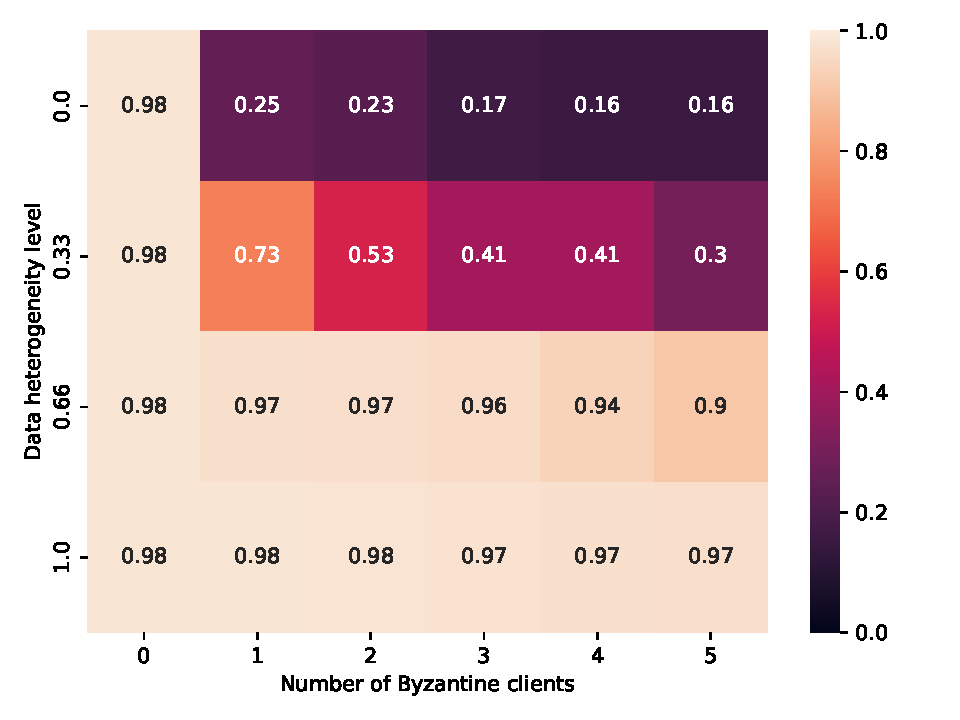
\includegraphics[width=\textwidth]{../plots/robust_comparison_sweep/learning_rate_0.1/best_test_mnist_cnn_mnist_gamma_similarity_niid_NNM_ARC_nb_honest_clients_10_tolerated_f_equal_real.pdf}
        \caption{$\text{LR} = 0.1$}
        \label{fig:best_overall_lr_0_1}
    \end{subfigure}
    \vspace{0.2cm}
    \begin{subfigure}[b]{0.24\textwidth}
        \centering
        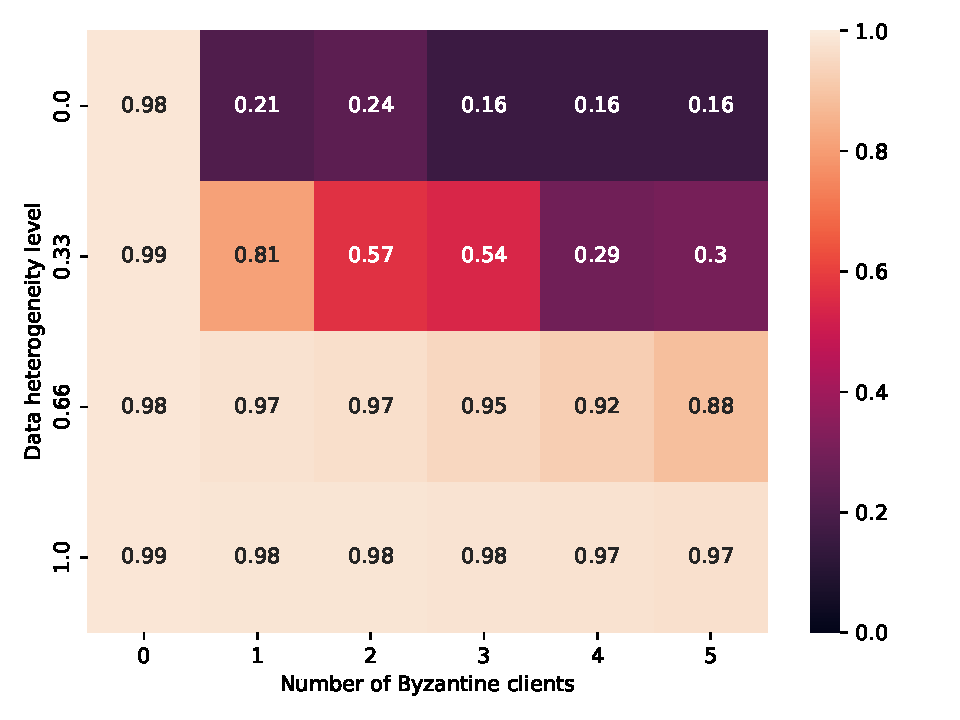
\includegraphics[width=\textwidth]{../plots/robust_comparison_sweep/learning_rate_0.12/best_test_mnist_cnn_mnist_gamma_similarity_niid_NNM_ARC_nb_honest_clients_10_tolerated_f_equal_real.pdf}
        \caption{$\text{LR} = 0.12$}
        \label{fig:best_overall_lr_0_12}
    \end{subfigure}
    \hfill
    \begin{subfigure}[b]{0.24\textwidth}
        \centering
        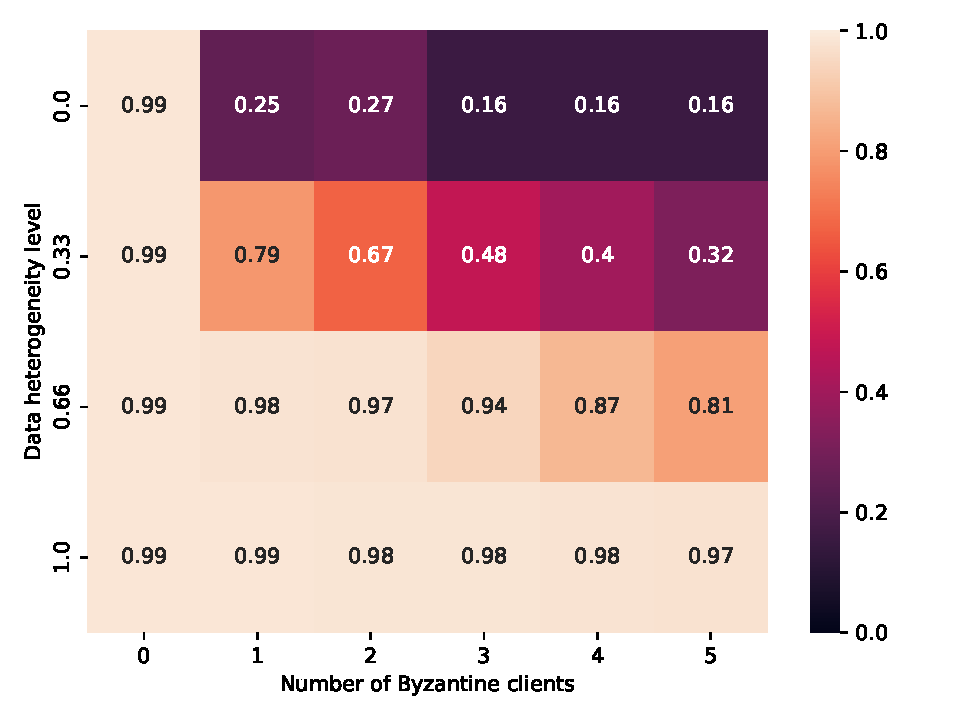
\includegraphics[width=\textwidth]{../plots/robust_comparison_sweep/learning_rate_0.15/best_test_mnist_cnn_mnist_gamma_similarity_niid_NNM_ARC_nb_honest_clients_10_tolerated_f_equal_real.pdf}
        \caption{$\text{LR} = 0.15$}
        \label{fig:best_overall_lr_0_15}
    \end{subfigure}
    \caption{Best overall test accuracy heatmaps (worst-case across attacks) for different learning rates.}
    \label{fig:best_overall_grid}
\end{figure}

\clearpage
\section{Best Aggregator under Specific Attacks}

\subsection{Optimal A Little Is Enough (ALIE) Attack}
\begin{figure}[htbp]
    \centering
    \begin{subfigure}[b]{0.24\textwidth}
        \centering
        \includegraphics[width=\textwidth]{../plots/robust_comparison_sweep/learning_rate_0.01/best_test_Optimal_ALittleIsEnough_neg1_mnist_cnn_mnist_gamma_similarity_niid_NNM_ARC_nb_honest_clients_10_tolerated_f_equal_real.pdf}
        \caption{$\text{LR} = 0.01$}
        \label{fig:best_alie_lr_0_01}
    \end{subfigure}
    \hfill
    \begin{subfigure}[b]{0.24\textwidth}
        \centering
        \includegraphics[width=\textwidth]{../plots/robust_comparison_sweep/learning_rate_0.05/best_test_Optimal_ALittleIsEnough_neg1_mnist_cnn_mnist_gamma_similarity_niid_NNM_ARC_nb_honest_clients_10_tolerated_f_equal_real.pdf}
        \caption{$\text{LR} = 0.05$}
        \label{fig:best_alie_lr_0_05}
    \end{subfigure}
    \hfill
    \begin{subfigure}[b]{0.24\textwidth}
        \centering
        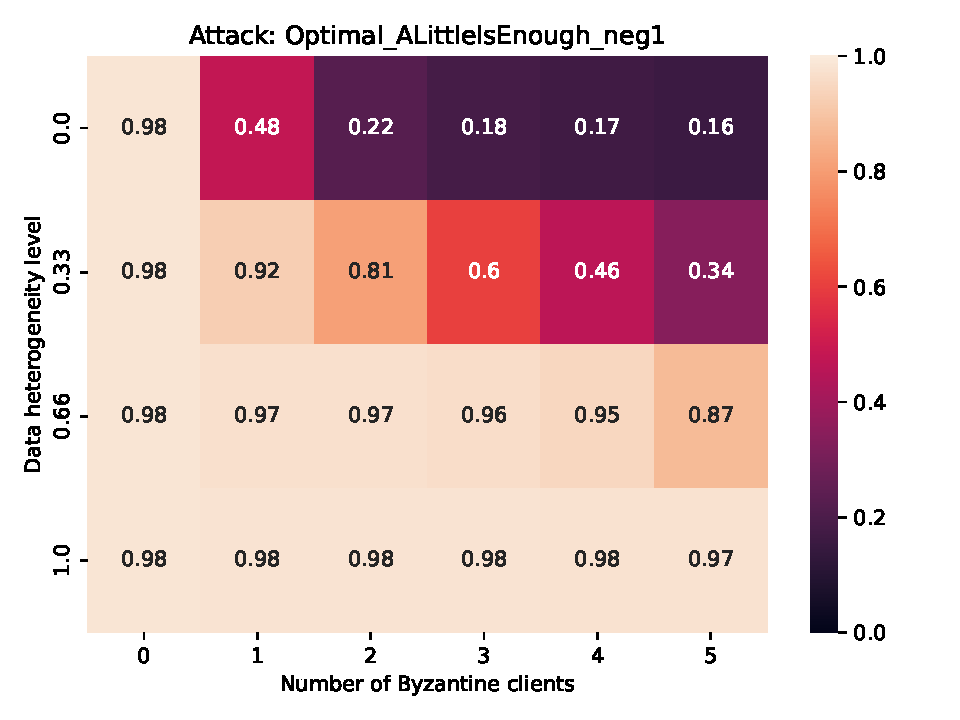
\includegraphics[width=\textwidth]{../plots/robust_comparison_sweep/learning_rate_0.08/best_test_Optimal_ALittleIsEnough_neg1_mnist_cnn_mnist_gamma_similarity_niid_NNM_ARC_nb_honest_clients_10_tolerated_f_equal_real.pdf}
        \caption{$\text{LR} = 0.08$}
        \label{fig:best_alie_lr_0_08}
    \end{subfigure}
    \hfill
    \begin{subfigure}[b]{0.24\textwidth}
        \centering
        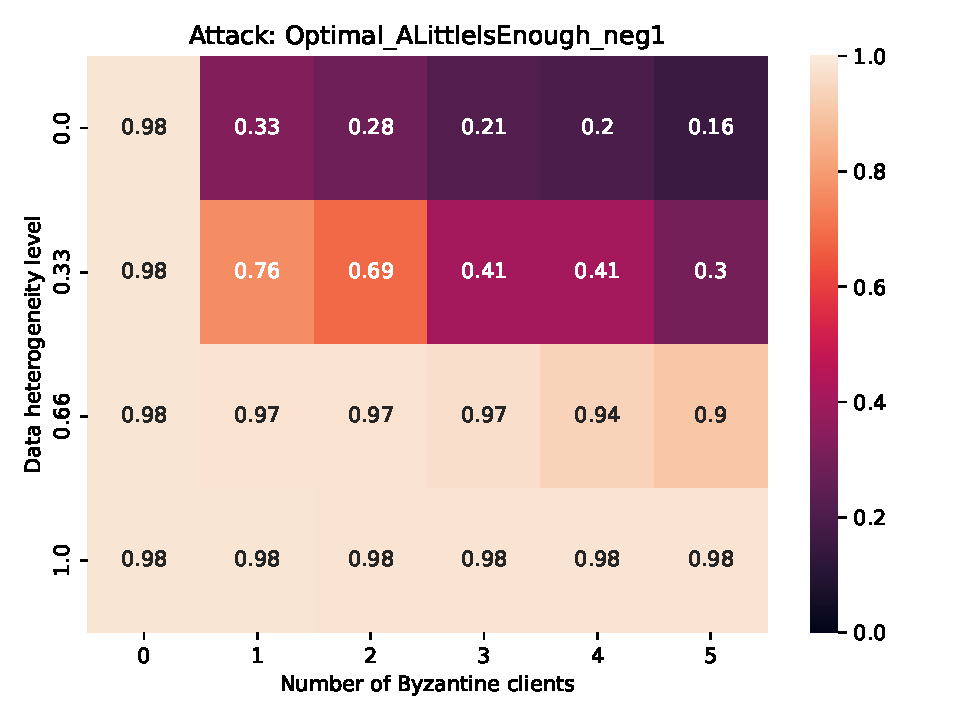
\includegraphics[width=\textwidth]{../plots/robust_comparison_sweep/learning_rate_0.1/best_test_Optimal_ALittleIsEnough_neg1_mnist_cnn_mnist_gamma_similarity_niid_NNM_ARC_nb_honest_clients_10_tolerated_f_equal_real.pdf}
        \caption{$\text{LR} = 0.1$}
        \label{fig:best_alie_lr_0_1}
    \end{subfigure}
    \vspace{0.2cm}
    \begin{subfigure}[b]{0.24\textwidth}
        \centering
        \includegraphics[width=\textwidth]{../plots/robust_comparison_sweep/learning_rate_0.12/best_test_Optimal_ALittleIsEnough_neg1_mnist_cnn_mnist_gamma_similarity_niid_NNM_ARC_nb_honest_clients_10_tolerated_f_equal_real.pdf}
        \caption{$\text{LR} = 0.12$}
        \label{fig:best_alie_lr_0_12}
    \end{subfigure}
    \hfill
    \begin{subfigure}[b]{0.24\textwidth}
        \centering
        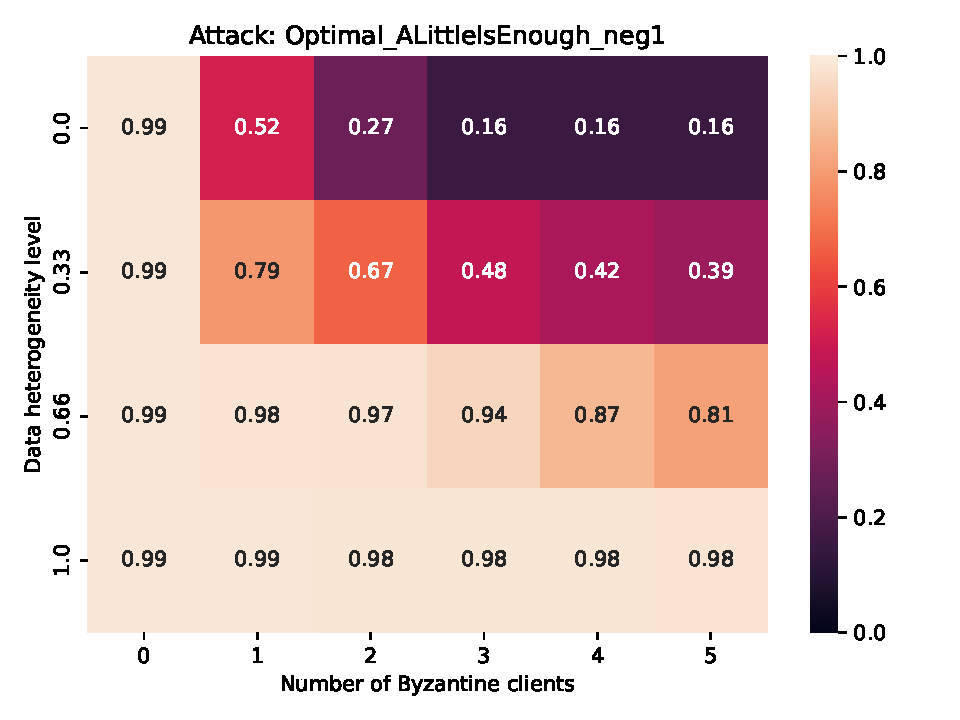
\includegraphics[width=\textwidth]{../plots/robust_comparison_sweep/learning_rate_0.15/best_test_Optimal_ALittleIsEnough_neg1_mnist_cnn_mnist_gamma_similarity_niid_NNM_ARC_nb_honest_clients_10_tolerated_f_equal_real.pdf}
        \caption{$\text{LR} = 0.15$}
        \label{fig:best_alie_lr_0_15}
    \end{subfigure}
    \caption{Best test accuracy heatmaps under the Optimal ALIE attack for different learning rates.}
    \label{fig:best_alie_grid}
\end{figure}
\clearpage
\subsection{Sign Flipping Attack}
\begin{figure}[htbp]
    \centering
    \begin{subfigure}[b]{0.24\textwidth}
        \centering
        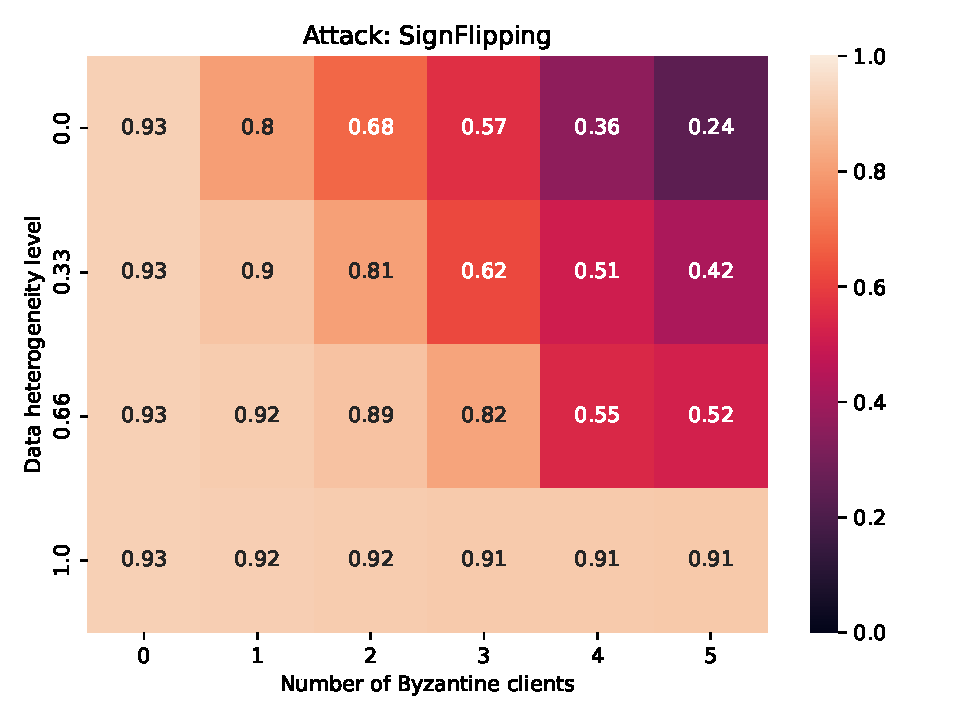
\includegraphics[width=\textwidth]{../plots/robust_comparison_sweep/learning_rate_0.01/best_test_SignFlipping_mnist_cnn_mnist_gamma_similarity_niid_NNM_ARC_nb_honest_clients_10_tolerated_f_equal_real.pdf}
        \caption{$\text{LR} = 0.01$}
        \label{fig:best_sf_lr_0_01}
    \end{subfigure}
    \hfill
    \begin{subfigure}[b]{0.24\textwidth}
        \centering
        \includegraphics[width=\textwidth]{../plots/robust_comparison_sweep/learning_rate_0.05/best_test_SignFlipping_mnist_cnn_mnist_gamma_similarity_niid_NNM_ARC_nb_honest_clients_10_tolerated_f_equal_real.pdf}
        \caption{$\text{LR} = 0.05$}
        \label{fig:best_sf_lr_0_05}
    \end{subfigure}
    \hfill
    \begin{subfigure}[b]{0.24\textwidth}
        \centering
        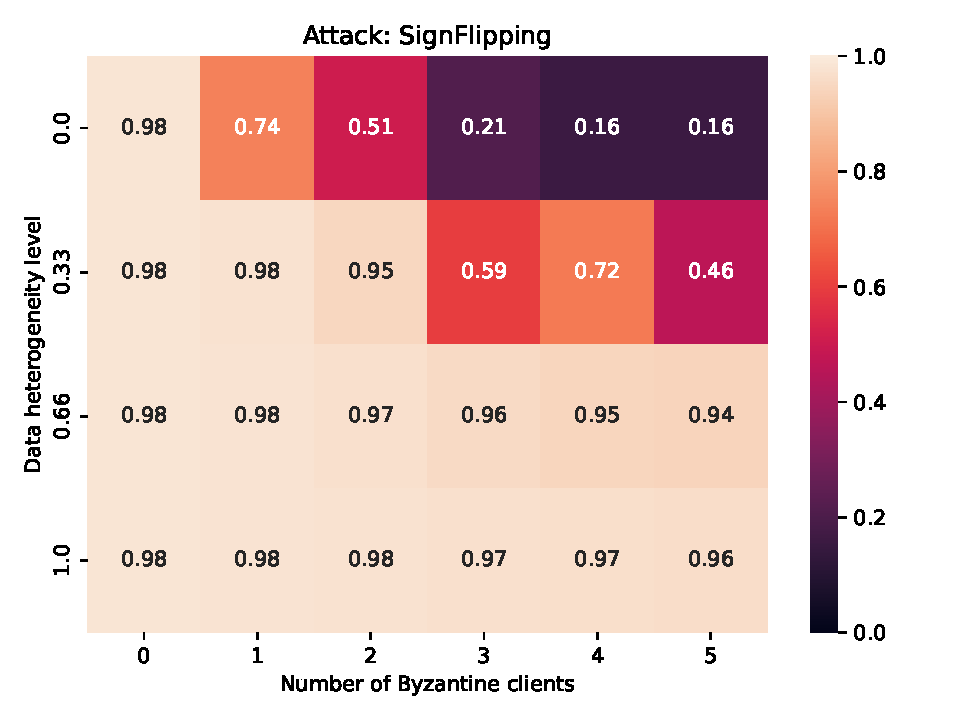
\includegraphics[width=\textwidth]{../plots/robust_comparison_sweep/learning_rate_0.08/best_test_SignFlipping_mnist_cnn_mnist_gamma_similarity_niid_NNM_ARC_nb_honest_clients_10_tolerated_f_equal_real.pdf}
        \caption{$\text{LR} = 0.08$}
        \label{fig:best_sf_lr_0_08}
    \end{subfigure}
    \hfill
    \begin{subfigure}[b]{0.24\textwidth}
        \centering
        \includegraphics[width=\textwidth]{../plots/robust_comparison_sweep/learning_rate_0.1/best_test_SignFlipping_mnist_cnn_mnist_gamma_similarity_niid_NNM_ARC_nb_honest_clients_10_tolerated_f_equal_real.pdf}
        \caption{$\text{LR} = 0.1$}
        \label{fig:best_sf_lr_0_1}
    \end{subfigure}
    \vspace{0.2cm}
    \begin{subfigure}[b]{0.24\textwidth}
        \centering
        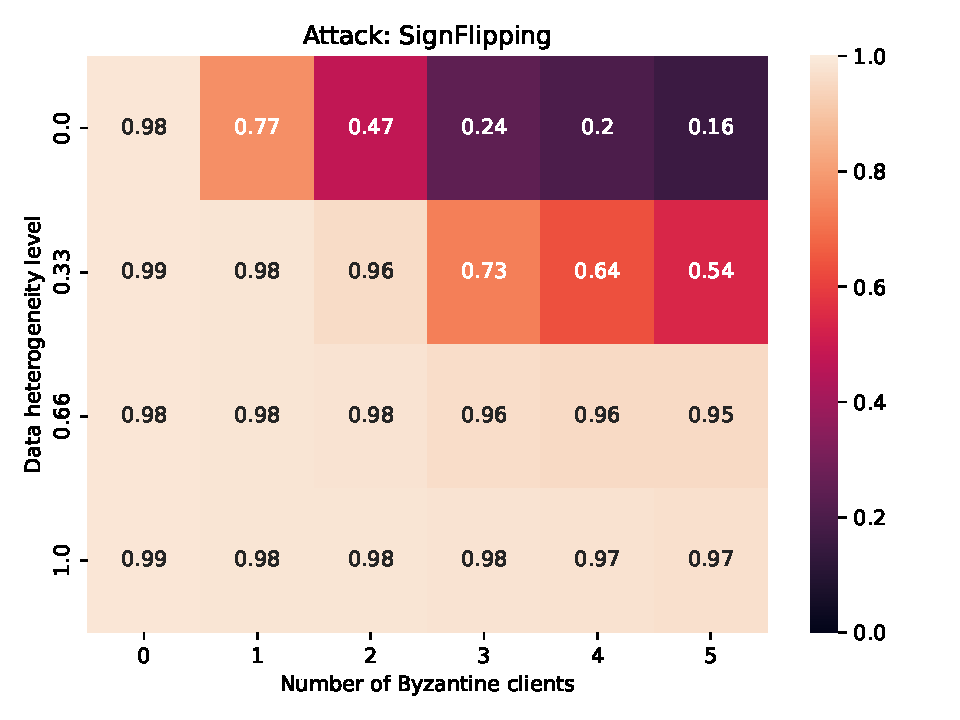
\includegraphics[width=\textwidth]{../plots/robust_comparison_sweep/learning_rate_0.12/best_test_SignFlipping_mnist_cnn_mnist_gamma_similarity_niid_NNM_ARC_nb_honest_clients_10_tolerated_f_equal_real.pdf}
        \caption{$\text{LR} = 0.12$}
        \label{fig:best_sf_lr_0_12}
    \end{subfigure}
    \hfill
    \begin{subfigure}[b]{0.24\textwidth}
        \centering
        \includegraphics[width=\textwidth]{../plots/robust_comparison_sweep/learning_rate_0.15/best_test_SignFlipping_mnist_cnn_mnist_gamma_similarity_niid_NNM_ARC_nb_honest_clients_10_tolerated_f_equal_real.pdf}
        \caption{$\text{LR} = 0.15$}
        \label{fig:best_sf_lr_0_15}
    \end{subfigure}
    \caption{Best test accuracy heatmaps under the Sign Flipping attack for different learning rates.}
    \label{fig:best_sf_grid}
\end{figure}
\clearpage
\subsection{Optimal Inner Product Manipulation Attack}
\begin{figure}[htbp]
    \centering
    \begin{subfigure}[b]{0.24\textwidth}
        \centering
        \includegraphics[width=\textwidth]{../plots/robust_comparison_sweep/learning_rate_0.01/best_test_Optimal_InnerProductManipulation_mnist_cnn_mnist_gamma_similarity_niid_NNM_ARC_nb_honest_clients_10_tolerated_f_equal_real.pdf}
        \caption{$\text{LR} = 0.01$}
        \label{fig:best_ipm_lr_0_01}
    \end{subfigure}
    \hfill
    \begin{subfigure}[b]{0.24\textwidth}
        \centering
        \includegraphics[width=\textwidth]{../plots/robust_comparison_sweep/learning_rate_0.05/best_test_Optimal_InnerProductManipulation_mnist_cnn_mnist_gamma_similarity_niid_NNM_ARC_nb_honest_clients_10_tolerated_f_equal_real.pdf}
        \caption{$\text{LR} = 0.05$}
        \label{fig:best_ipm_lr_0_05}
    \end{subfigure}
    \hfill
    \begin{subfigure}[b]{0.24\textwidth}
        \centering
        \includegraphics[width=\textwidth]{../plots/robust_comparison_sweep/learning_rate_0.08/best_test_Optimal_InnerProductManipulation_mnist_cnn_mnist_gamma_similarity_niid_NNM_ARC_nb_honest_clients_10_tolerated_f_equal_real.pdf}
        \caption{$\text{LR} = 0.08$}
        \label{fig:best_ipm_lr_0_08}
    \end{subfigure}
    \hfill
    \begin{subfigure}[b]{0.24\textwidth}
        \centering
        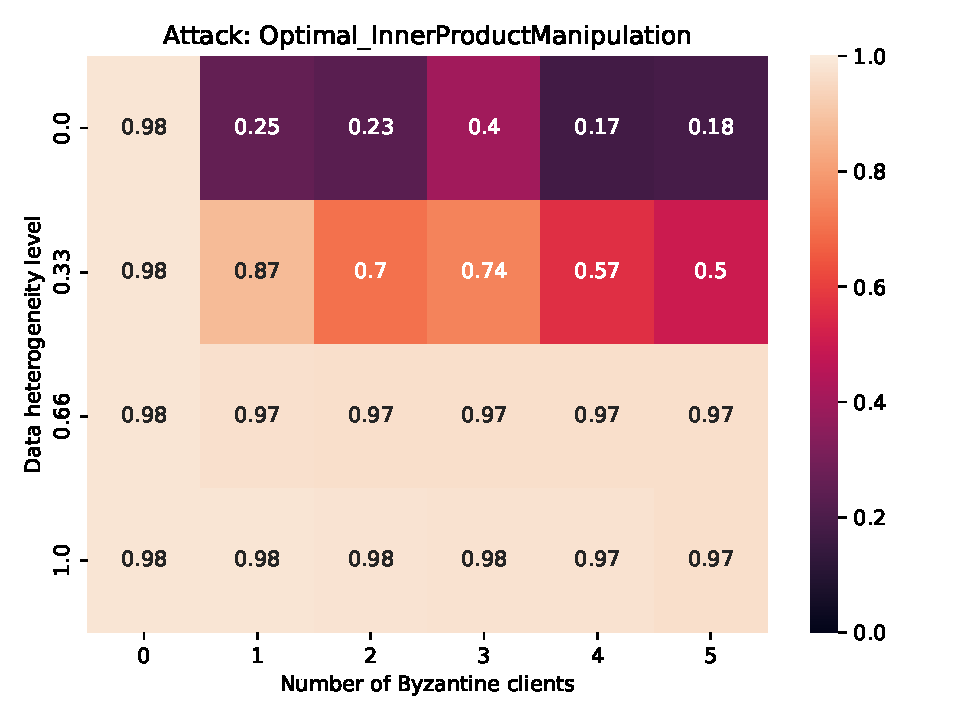
\includegraphics[width=\textwidth]{../plots/robust_comparison_sweep/learning_rate_0.1/best_test_Optimal_InnerProductManipulation_mnist_cnn_mnist_gamma_similarity_niid_NNM_ARC_nb_honest_clients_10_tolerated_f_equal_real.pdf}
        \caption{$\text{LR} = 0.1$}
        \label{fig:best_ipm_lr_0_1}
    \end{subfigure}
    \vspace{0.2cm}
    \begin{subfigure}[b]{0.24\textwidth}
        \centering
        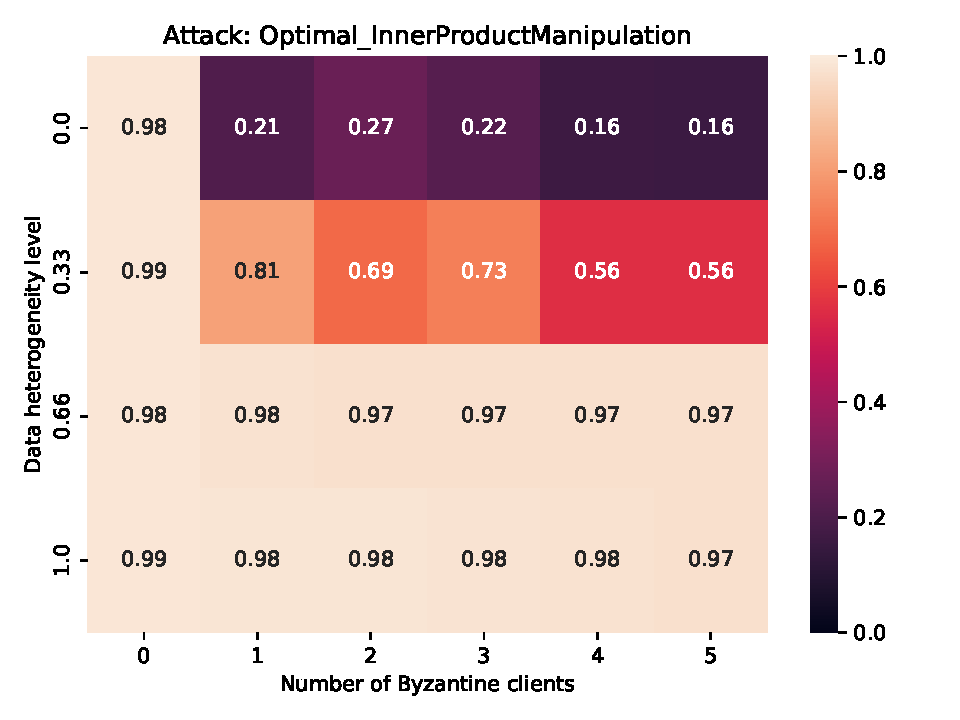
\includegraphics[width=\textwidth]{../plots/robust_comparison_sweep/learning_rate_0.12/best_test_Optimal_InnerProductManipulation_mnist_cnn_mnist_gamma_similarity_niid_NNM_ARC_nb_honest_clients_10_tolerated_f_equal_real.pdf}
        \caption{$\text{LR} = 0.12$}
        \label{fig:best_ipm_lr_0_12}
    \end{subfigure}
    \hfill
    \begin{subfigure}[b]{0.24\textwidth}
        \centering
        \includegraphics[width=\textwidth]{../plots/robust_comparison_sweep/learning_rate_0.15/best_test_Optimal_InnerProductManipulation_mnist_cnn_mnist_gamma_similarity_niid_NNM_ARC_nb_honest_clients_10_tolerated_f_equal_real.pdf}
        \caption{$\text{LR} = 0.15$}
        \label{fig:best_ipm_lr_0_15}
    \end{subfigure}
    \caption{Best test accuracy heatmaps under the Optimal Inner Product Manipulation attack for different learning rates.}
    \label{fig:best_ipm_grid}
\end{figure}
\end{document}
